\documentclass[12pt]{article}
\usepackage{graphicx}
\usepackage{enumitem}
\usepackage{multicol}
\usepackage{mathtools}
\usepackage[margin=1in]{geometry}
\usepackage{amsmath,amsthm,amssymb}

 
\begin{document}
 
% --------------------------------------------------------------
%                         Start here
% --------------------------------------------------------------
 
\title{AST1430 Assignment 1}
\author{Jessica Campbell}
\date{February 9, 2018}
\maketitle

% --------------------------------------------------------------
%               1. Textbook Questions
% --------------------------------------------------------------

\section{Textbook Questions (not to be handed in)}

Work through all problems in Chapter 1 of RL. Consult the solutions (end of book) if you get stuck. Make sure that you are proficient at these.

% --------------------------------------------------------------
%                    2. Photosphere
% --------------------------------------------------------------
\section{Photosphere}

The temperature inside a star goes from a few million kelvins (interior) to practically zero (outside). On Earth ($\tau=0$), we observe a radiation spectrum that is characterized by a temperature called the ’effective temperature’ and is measured at an optical depth of order unity (photosphere).\\

\subsection*{Part 1}

{\noindent}Show that the bolometric flux radiated outward per unit area by a blackbody with temperature $T$ is $F = {\pi}{\int}S_{\nu}d_{\nu}$ and is ${\sigma}T^4$.

\subsection*{Solution}

\begin{equation*}
\begin{split}
F &= \int F_\nu d\nu = \int I_\nu \cos \theta d\Omega = \int_{0}^{\infty}I_\nu d\nu \int_0^{\pi/2}\cos\theta\sin\theta d\theta \int_0^{2\pi}d\phi \\
&= \int_0^{\infty}I_\nu d\nu \int_0^{\pi/2}\frac{1}{2}\sin2\theta d\theta \int_0^{2\pi}d\phi = \int_0^{\infty}I_\nu d\nu \left[-\frac{1}{2}\frac{1}{2}\cos2\theta\right]_0^{\pi/2}[\phi]_0^{2\pi} \\
&= -\frac{1}{4}\int_0^{\infty}I_\nu d\nu[\cos\pi - \cos0][2\pi] = \frac{1}{2}\int_0^{\infty}I_\nu d\nu[1+1][\pi] = \pi\int_0^{\infty}I_\nu d\nu
\end{split}
\end{equation*}

For optically thick media $(\tau \gg 1)$, $I_\nu \rightarrow S_\nu$. Thus,

\begin{align*}
F = \pi\int_0^{\infty}S_\nu d\nu.
\end{align*}

For thermal radiation, $S_\nu \rightarrow B_\nu(T)$, so:

\begin{equation*}
\begin{split}
F &= \pi\int_0^{\infty}S_\nu d\nu = \pi\int_0^{\infty}B_\nu(T) d\nu = \pi\int_0^{\infty}\frac{2h\nu^3}{c^2}\frac{1}{\mathrm{exp}(h\nu/k_BT) - 1}d\nu \\
&= \frac{2\pi h}{c^2}\int_0^{\infty}\frac{\nu^3}{\mathrm{exp}(h\nu/K_BT)-1}d\nu.
\end{split}
\end{equation*}

Let $x\equiv(h\nu/k_BT)$ such that $\nu = x(k_BT/h)$. Then,

\begin{equation*}
\begin{split}
F &= \frac{2\pi h}{c^2}\int_0^{\infty}\frac{(xk_BT/h)^3}{\mathrm{exp}(x)-1}dx = \frac{2\pi h}{c^2}\left(\frac{k_BT}{h}\right)^4\int_0^{\infty}\frac{x}{\mathrm{exp}(x)-1}dx \\
&= \frac{2\pi k_BT^4}{c^2h^3}\int_0^{\infty}\frac{x}{\mathrm{exp}(x)-1}dx = \frac{2\pi k_BT^4}{c^2h^3}\left[\frac{\pi^4}{15}\right] = \left(\frac{2\pi^5k_B}{15c^2h^3}\right)T^4.
\end{split}
\end{equation*}

Therefore,

$F = \sigma T^4$ where $\sigma \equiv \left(\frac{2\pi^5k_B}{15c^2h^3}\right)$ is Boltzmann's constant.

\subsection*{Part 2}

In the case of a stellar atmosphere, show that the observed flux $F_\nu(\tau_\nu = 0) = {\pi}S_{\nu}(\tau_{\nu} = 2/3)$ (also called the Eddington-Barbier approximation), namely, the photospheric optical depth is 2/3. We suppress all $\nu$ subscript from now on. To accomplish this (in a cheap way), start from the equation of radiative transfer in plane-parallel atmosphere (RL eq. [1.116]). Taylor expand the source function $S_\tau$ around small $\tau$, and iteratively solve the above equation to obtain $I(\tau=0,\mu) = S(\tau = \mu)$. Obtain the corresponding $F(\tau=0)$.

\subsection*{Solution}

The equation of radiative transfer in a plane-parallel atmosphere is as follows:

\begin{align*}
\mu\frac{\partial I}{\partial \tau} = I - S
\end{align*}

which can be rewritten as:

\begin{align*}
I = S + \mu\frac{\partial I}{\partial \tau}.
\end{align*}

Taylor expanding $S(\tau)$ around $\tau \ll 1$:

\begin{align*}
S(\tau) \approx S_0 + S_1\tau + S_2\tau^2.
\end{align*}

Using the Taylor expansion of $S(\tau)$ for our initial guess $I_0$:

\begin{align*}
I_0 \approx S(\tau) = S_0 + S_1\tau + S_2\tau^2.
\end{align*}

\begin{align*}
\frac{\partial I_0}{\partial \tau} = \frac{\partial}{\partial \tau}(S_0 + S_1\tau + S_2\tau^2) = S_1 + 2S_2\tau.
\end{align*}

Plugging this back into our radiative transfer equation for our refined guess $I_1$...

\begin{align*}
I_1 = S(\tau) + \mu\frac{\partial I_0}{\partial \tau} = (S_0 + S_1\tau + S_2\tau^2) + \mu(S_1 + 2S_2\tau) = (S_0+\mu S_1) + (S_1+2\mu S_2)\tau + S_2\tau^2.
\end{align*}

\begin{align*}
\frac{\partial I_1}{\partial \tau} = \frac{\partial}{\partial \tau}\left[(S_0 + S_1\tau + S_2\tau^2) + \mu(S_1 + 2S_2\tau)\right] = (S_1+2\mu S_2) + 2S_2\tau.
\end{align*}

Plugging this back into our radiative transfer equation for our refined guess $I_2$...

\begin{equation*}
\begin{split}
I_2 &= S(\tau) + \mu\frac{\partial I_1}{\partial \tau} = (S_0 + S_1\tau + S_2\tau^2) + \mu\left[(S_1+2\mu S_2) + 2S_2\tau\right] \\
&= (S_0+S_1 \mu+2\mu^2S_2) + (S_1+2\mu S_2)\tau + S_2\tau^2.
\end{split}
\end{equation*}

\begin{align*}
\frac{\partial I_2}{\partial \tau} = \frac{\partial}{\partial \tau}\left[(S_0+S_1 \mu+2\mu^2S_2) + (S_1+2\mu S_2)\tau + S_2\tau^2\right] = (S_1+2\mu S_2) + 2S_2\tau.
\end{align*}

Plugging this back into our radiative transfer equation for our refined guess $I_3$...

\begin{equation*}
\begin{split}
I_3 &= S(\tau) + \mu\frac{\partial I_2}{\partial \tau} = (S_0 + S_1\tau + S_2\tau^2) + \mu\left[(S_1+2\mu S_2) + 2S_2\tau\right] \\
&= (S_0+S_1 \mu+2\mu^2S_2) + (S_1+2\mu S_2)\tau + S_2\tau^2.
\end{split}
\end{equation*}

This is the same as $I_2$ so we have reached our solution:

\begin{align*}
I = (S_0+S_1 \mu+2\mu^2S_2) + (S_1+2\mu S_2)\tau + S_2\tau^2.
\end{align*}

Given this solution, $I(\tau=0,\mu) = S_0 +\mu S_1 + 2\mu^2 S_2$ is consistent with $(\tau=\mu) = S_0 + \mu S_1 + \mu^2S_2$.

\subsection*{Part 3}

Use result in 2) to explain ’Limb Darkening’. Under what condition would you get ’Limb Brightening’ instead?

\subsection*{Solution}

When observing the specific intensity $I_\nu$ across the solar disk, we are seeing different depths into the atmosphere (and therefore different temperatures) because the optical depth $\tau$ varies across the solar disk. Near the disk centre, the optical depth is higher $(\tau \sim 1)$ so we are seeing deeper into the iterior where the temperature is hotter and brightness is greater. Towards the disk edges, the optical depth decreases so we are seeing higher elevations in the solar atmosphere where the temperature is cooler and brightness is lower. As we csn dee from Part 2, the specific intensity depends on the optical depth in such a way that decreasing $\tau \rightarrow$ decreasing $I$ towards the solar edges. This is "limb darkening." In order to get "limb brightening," the temperature would need to increase with elevation such that the brightness would increase with decreasing optical depths. Such a scenario is believed to occur in the solar corona where the temperature drastically increases beyond the photosphere.

% --------------------------------------------------------------
%                    3. Photon Pressure
% --------------------------------------------------------------

\section{Photon Pressure}

If photon momentum is related to energy as $p = \frac{3}{4}h\nu/c$ (an extra factor 3/4 compared to the real one), rederive the expressions for radiation pressure (RL eq. [1.10]) and the Stefan-Boltzman law (RL eq. [1.41]).

\subsection*{Solution}

{\noindent}\textbf{Radiation pressure:}
\begin{align*}
p_\nu[\mathrm{dynes\cdot cm^{-2}}] = \frac{3}{4}\frac{1}{c}\int I_\nu\cos^2\theta d\Omega.
\end{align*}

For a reflecting enclosure containing an isotropic radiation field, each photon transfers twice its normal component of momentum upon reflection:

\begin{align*}
p_\nu = (2)\frac{3}{4}\frac{1}{c}\int I_\nu\cos^2\theta d\Omega = \frac{3}{2c}\int I_\nu\cos^2\theta d\Omega.
\end{align*}

For isotropic radiation, $I_\nu = J_\nu (\equiv \frac{1}{4\pi}\int I_\nu d\nu)$, so:

\begin{align*}
\frac{3}{2c}\int_0^{\infty} J_\nu \int_0^{\pi/2}\cos^2\theta\sin\theta d\theta \int_0^{2\pi} d\phi.
\end{align*}

Since the radiation energy density is $u = \int_0^{\infty}u_\nu d\nu = \frac{4\pi}{c}\int_0^{\infty}J_\nu d\nu$, we can make the substitution $\int_0^{\infty}J_\nu d\nu = \left(\frac{c}{4\pi}\right)u$:

\begin{align*}
p = \frac{3}{2c}\left[\frac{c}{4\pi}u\right]\left[-\frac{1}{3}\cos^3\theta\right]_0^{\pi/2}\left[2\pi\right]_0^{2\pi} = \frac{u}{4}.
\end{align*}

Therefore $p = u/4$ is the radiation pressure.

{\noindent}\textbf{Stefan-Boltzmann Law:}

The first law of thermodynamics is $dQ = dU + pdV$ while the second law of thermodynamics: $dS = dQ/T$, where $U=uV$, $p=u/4$, and $u = (4\pi/c)\int J_\nu d\nu$; $S$ is entropy, $Q$ is heat, $T$ is temperature, $U$ is total energy, $p$ is radiation pressure, and $V$ is volume. Starting with the second law of thermodynamics:

\begin{equation*}
\begin{split}
dS &= \frac{dQ}{T} = \frac{(dU+pdV)}{T} = \frac{d(uV)+pdV}{T} = \frac{Vdu+udV+pdV}{T} \\
&= \frac{V}{T}\frac{dU}{dT}dT + \frac{u}{T}dV + \left(\frac{1}{4}\frac{u}{T}\right)dV = \frac{V}{T}\frac{dU}{dT}dT + \frac{5}{4}\frac{u}{T}dV.
\end{split}
\end{equation*}

The entropy $S$ therefore has the following partial derivatives:

\begin{align*}
\left(\frac{\partial S}{\partial T}\right)_V = \frac{V}{T}\frac{du}{dT}, \left(\frac{\partial S}{\partial V}\right)_T = \frac{5u}{4T}.
\end{align*}

Using Clairaut's Theorem, we can now write the second partial derivatives of entropy as:

\begin{align*}
\frac{\partial^2S}{\partial T \partial V} = \frac{\partial}{\partial T}\left(\frac{\partial S}{\partial V}\right)_T = \frac{\partial}{\partial V}\left(\frac{\partial S}{\partial T}\right)_V.
\end{align*}

Substituting the partial derivatives from above, we can solve the partial differential equation for the new Stefan-Boltzmann relation:

\begin{equation*}
\begin{split}
\frac{\partial}{\partial T}\left(\frac{5u}{4T}\right) &= \frac{\partial}{\partial V}\left(\frac{V}{T}\frac{du}{dT}\right)\\
\frac{5}{4}\frac{\partial}{\partial T}(uT^{-1}) &= \frac{1}{T}\frac{du}{dT}\frac{\partial}{\partial V}\left(V\right)\\
\frac{5}{4}\frac{\partial}{\partial T}(\frac{1}{T}\frac{\partial}{\partial T}u + u\frac{\partial}{\partial T}T^{-1}) &= \frac{1}{T}\frac{du}{dT}\\
\frac{5}{4}\left(\frac{1}{T}\frac{du}{dT} - \frac{u}{T^2}\right) &= \frac{1}{T}\frac{du}{dT}\\
\frac{5}{4}\left(\frac{du}{dT} - \frac{u}{T}\right) &= \frac{du}{dT} \\
\frac{du}{dT}\left(\frac{5}{4}-1\right) &= \frac{5}{4}\frac{u}{T}\\
\frac{du}{u} &= 5\frac{dT}{T}\\
\int\frac{du}{u} &= 5\int\frac{dT}{T}\\
ln(u) &= 5ln(T) + ln(c)\\
e^{ln(u)} &= e^{5ln(T)}e^{ln(c)}\\
u &= cT^5,
\end{split}
\end{equation*}

where $c$ is an integration constant.

% --------------------------------------------------------------
%                    4. Photon Pressure
% --------------------------------------------------------------

\section{The Greenhouse Effect}

The Sun heats the Earth. One can derive an equilibrium temperature for an air-less Earth $T_p$ assuming energy conservation and a black-body surface. This has to
be modified when an atmosphere exists. The earth atmosphere is optically thin in the visible wavelengths so the solar radiation hits the ground directly. However, it is optically thick in the infra-red wavelengths and intercepts radiation from the ground. The heat is eventually lost to the vacuum as the atmosphere radiates with an effective temperature $T_{eff}$. Necessarily, $T_{eff} = T_p$ (think why).

\subsection*{Part 1}

Imagine the atmosphere as a single opaque layer with a uniform temperature $T_p$. It is receiving heat from the ground $(T_g)$ and radiates as much luminosity toward the ground as towards the vacuum outside. Use energy conservation to show that $T_g = 2^{1/4}T_p$. So the ground has to be hotter.

\subsection*{Solution}

Figure \ref{fig:greenhouse} depicts the flow of radiative flux between the Earth, atmosphere and space:

\begin{figure}[h] \label{fig:greenhouse}
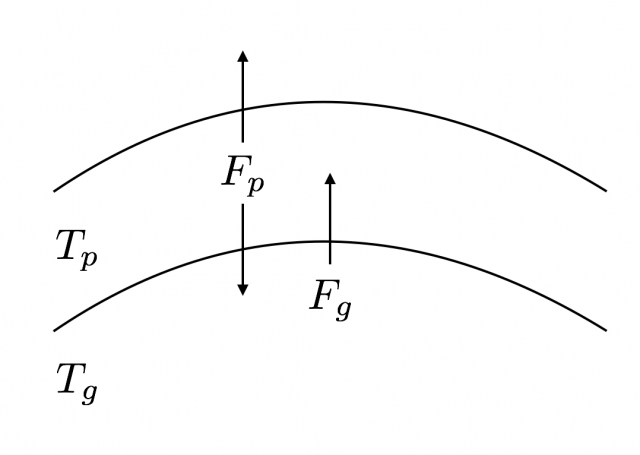
\includegraphics[width=8cm]{greenhouse.png}
\centering
\caption{Radiative conservation for the Earth's atmosphere.}
\end{figure}

In thermal equilibrium, the radiative flux entering the atmosphere must equal that exiting the atmosphere:

\begin{equation*}
\begin{split}
F_{in} &= F_{out}\\
F_g &= 2 F_p\\
(\sigma T_g^4) &= 2 (\sigma T_p^4)\\
T_g &= 2^{1/4}T_p.
\end{split}
\end{equation*}

\subsection*{Part 2}

A more sophisticated approach is to allow different layers in the atmosphere to have different temperatures. Let $\tau_g$ be the optical depth (to outgoing radiation) measured at the ground, while $\tau = 2/3$ at the photosphere (problem 2). Use the radiative diffusion equation (RL eq. [1.111]) to show that

\begin{align*}
T_g^4 = T_p^4 = \left[ 1 + \frac{3}{4} \left( \tau_g - \frac{2}{3} \right) \right].
\end{align*}

This reduces to the result in Part 1 when $\tau_g = 2.$

\subsection*{Solution}

The one-dimensional radiative diffusion equation reads:

\begin{align*}
F(z) = \frac{16\sigma T^3}{3\alpha_R}\frac{dT}{dz},
\end{align*}

where since $d\tau = \alpha_Rdz$, we can use the fact that $dz = d\tau/\alpha_R$:

\begin{equation*}
\begin{split}
F_{rad} &= \frac{16\sigma T^3}{3\alpha_R}\frac{dT}{(d\tau/\alpha_R)}\\
F_{rad} &= \frac{16\sigma T^3}{3\alpha_R}\frac{dT}{(d\tau/\alpha_R)}\\
F_{rad} &= \frac{16\sigma T^3}{3}\frac{dT}{d\tau}.
\end{split}
\end{equation*}

Since this $F_{rad}$ must equal $F_p = \sigma T_p^4$:

\begin{equation*}
\begin{split}
\sigma T_p^4 &= \frac{16\sigma T^3}{3}\frac{dT}{d\tau}\\
T_p^4d\tau &= \frac{16}{3}T^3dT\\
T_p^4\int_{\tau_g}^{2/3}d\tau &= \frac{16}{3}\int_{T_g}^{T_p}T^3dT\\
T_p^4[\tau]_{\tau_g}^{2/3} &= \frac{16}{3}\left[\frac{T^4}{4}\right]_{T_g}^{T_p}\\
T_p^4(\frac{2}{3} - \tau_g) &= \frac{4}{3}(T_p^4 - T_g^4)\\
T_g^4 &= T_p^4 - \frac{3}{4}T_p^4(\frac{2}{3} - \tau_g)\\
T_g^4 &= T_p^4\left[1 + \frac{3}{4}(\tau_g - \frac{2}{3})\right].
\end{split}
\end{equation*}

When $\tau_g = 2$,

\begin{equation*}
\begin{split}
T_g^4 &= T_p^4\left[1 + \frac{3}{4}(2 - \frac{2}{3})\right]\\
T_g^4 &= 2T_p^4\\
T_g &= 2^{1/4}T_p.
\end{split}
\end{equation*}

\subsection*{Part 3}

The opacity used above is the so-called Rosseland mean opacity (RL eq. [1.110]). What chemical species (atoms, molecules, aerosols...) are most relevant for determining this opacity? In contrast, what is the dominant opacity source in the visible wavelengths?

\subsection*{Solution}

The dominant chemical species for determining the Rosseland mean opacity for the Earth's atmosphere are: water $\mathrm{(H_2O)}$, carbon monoxide $\mathrm{(CO)}$, and methane $\mathrm{(CH_4)}$. In the visible wavelengths, there is water vapour (i.e., clouds) and Rayleigh scattering.

\section{Equivalent Width and Curve of Growth Analysis}

This problem is based on the data of Roberge et al (2004, Nature, 441, 72, also comes with supplementary material). The aim is to determine the range of uncertainty in the values for the atomic column densities obtained from absorption spectra.

\subsection*{Part 1}

First extract from the NIST database (http://physics.nist.gov/PhysRefData/ASD, choose “lines”) Einstein A coefficient and statistical weights relevant for the following transitions: $\mathrm{CII} \, \lambda = 1036.34$ \AA \, line, $\mathrm{CII^*} \, \lambda = 1037.02$ \AA \, line, and $\mathrm{OI} \, \lambda = 976.45$ \AA \, line.

\subsection*{Solution}

\begin{figure}[h] \label{fig:table}
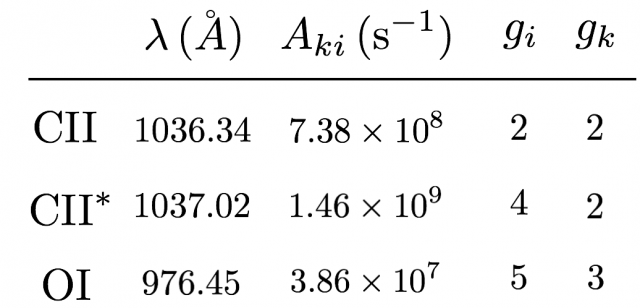
\includegraphics[width=8cm]{table.png}
\centering
\caption{NIST results.}
\end{figure}

\subsection*{Part 2}

Starting from eq. (1.78) in RL, obtain the following absorption coefficient $\alpha_\nu$,

\begin{equation*}
\begin{split}
\alpha_\nu = \frac{c^2}{8\pi\nu^2}n_aA_{21}\frac{g1}{g2}\left( 1 - \frac{g_1n_2}{g_2n_1}\right)\phi(\nu) = \frac{c^2}{8\pi\nu^2}n_aA_{21}\frac{g1}{g2}\left[ 1 - \mathrm{exp}\left(-\frac{{\Delta}E}{k_BT}\right)\right]\phi(\nu),
\end{split}
\end{equation*}

where ${\Delta}E$ is the transition energy, $T_s$ is the excitation temperature of atoms (see Problem 6) and for our problem here, the limit $k_BT_s \ll {\Delta}E$ applies.

\subsection*{Solution}

The equation for the absorption coefficient is:

\begin{align*}
\alpha_\nu = \frac{h\nu}{4\pi}n_1B_{12}\left(1 - \frac{g_1n_2}{g_2n_1}\right)\phi(\nu).
\end{align*}

We therefore need to start by finding $B_{12}$. Starting with the following detailed balance equations:

\begin{align*}
\frac{B_{12}}{B_{21}} = \frac{g_2}{g_1}, \frac{A_{21}}{B_{21}} = \frac{2h\nu^3}{c^2}
\end{align*}

we can solve for $B_{12}$ via

\begin{align*}
B_{12} = B_{21}\left(\frac{g_2}{g_1}\right)
\end{align*}

by plugging in the following for $B_{21}$:

\begin{align*}
B_{21} = A_{21}\left(\frac{c^2}{2h\nu^3}\right).
\end{align*}

Doing this, we obtain the following:

\begin{align*}
B_{12} = \left[A_{21}\frac{c^2}{2h\nu^3}\right]\left(\frac{g_2}{g_1}\right).
\end{align*}

Plugging this back into $\alpha_\nu$, we obtain:

\begin{equation*}
\begin{split}
\alpha_\nu &= \frac{h\nu}{4\pi}n_1\left[A_{21}\left(\frac{c^2}{2h\nu^3}\right)\left(\frac{g_2}{g_1}\right)\right]\left(1-\frac{g_1n_2}{g_2n_1}\right)\phi(\nu)
\alpha_\nu \\
&= \frac{c^2n_1}{8\pi \nu^2}A_{21}\left(\frac{g_2}{g_1}\right)\left(1-\frac{g_1n_2}{g_2n_1}\right)\phi(\nu).
\end{split}
\end{equation*}

We can now use the Boltzmann equation

\begin{align*}
\frac{n_1}{n_2} = \frac{g_1}{g_2}\mathrm{exp}\left(\frac{h\nu}{k_BT}\right)
\end{align*}

to solve for $(g_1n_1/g_2n_2)$:

\begin{align*}
\frac{g_1h_1}{g_2n_2} = \mathrm{exp}\left(-\frac{h\nu}{k_BT}\right).
\end{align*}

Substituting this back into our equation for $\alpha_\nu$ gives us the final form for the absorption coefficient:

\begin{equation*}
\begin{split}
\alpha_\nu &= \frac{c^2n_1}{8\pi \nu^2}A_{21}\left(\frac{g_2}{g_1}\right)\left[1-\mathrm{exp}\left(-\frac{h\nu}{k_BT}\right)\right]\phi(\nu) \\
 &= \frac{c^2n_1}{8\pi \nu^2}A_{21}\left(\frac{g_2}{g_1}\right)\left[1-\mathrm{exp}\left(-\frac{\Delta E}{k_BT_s}\right)\right]\phi(\nu)
\end{split}
\end{equation*}

where $\Delta E$ is the transition energy and $T_s$ is the excitation temperature.

In the limit where $k_BT_s \ll \Delta E$, this reduces to:

\begin{align*}
\alpha_\nu = \frac{c^2n_1}{8\pi \nu^2}A_{21}\left(\frac{g_2}{g_1}\right)\phi(\nu).
\end{align*}

\subsection*{Part 3}

Show that for all three transitions (ignore the broad, redshifted components for carbon), the sort of column density values as listed in their Table 1 would imply that optical depths at the line centres ($\tau_{\nu = \nu_0}$) are greater than or comparable to 1. Or, these lines are saturated. In the author's opinion, Doppler broadening is important for the line-width,

\begin{align*}
\phi(\nu) \frac{1}{\sqrt{\pi}\Delta\nu_D}\mathrm{exp}\left[-\left(\frac{\nu - \nu_0}{\Delta\nu_D}\right)^2\right]
\end{align*}

where $\Delta\nu_D$ is the line width and is related to the Doppler parameter $b$ (matter sound speed) as $\Delta\nu_D \approx (b/c)\nu_0$. Use the values for $b$ as listed in Table 1.

\subsection*{Solution}

Now that we have the equation for the absorption coefficient, let's start with the relation between optical depth and the absorption coefficient:

\begin{equation*}
\begin{split}
d\tau = \alpha_\nu ds
d\tau = \frac{c^2n_1}{8\pi \nu^2}A_{21}\left(\frac{g_2}{g_1}\right)\phi(\nu)ds
\int d\tau = \frac{c^2}{8\pi \nu^2}A_{21}\left(\frac{g_2}{g_1}\right)\phi(\nu)\int n_1ds.
\end{split}
\end{equation*}

Integrating and using the definition of column density, $N \equiv \int nds$,

\begin{align*}
\tau = \frac{c^2}{8\pi \nu^2}A_{21}N_1\left(\frac{g_2}{g_1}\right)\phi(\nu).
\end{align*}

Now, substituting the equation for a  Doppler broadened dominated line profile into $\phi(\nu)$:

\begin{align*}
\tau = \frac{c^2}{8\pi \nu^2}A_{21}N_1\left(\frac{g_2}{g_1}\right)\left[\frac{1}{\sqrt{\pi}\Delta\nu_D}\mathrm{exp}\left(-\frac{\nu-\nu_0}{\Delta\nu_D}\right)^2\right].
\end{align*}

Using the fact that $\Delta\nu_D \approx (b/c)\nu_0$ and letting $\nu \equiv \nu_0$:

\begin{equation*}
\begin{split}
\tau = \frac{c^2}{8\pi \nu_0^2}A_{21}N_1\left(\frac{g_2}{g_1}\right)\left[\frac{1}{\sqrt{\pi}(b/c)\nu_0}\mathrm{exp}(0)^2\right]
= \frac{c^2}{8\pi^{3/2}b\nu_0^3}A_{21}N_1\left(\frac{g_2}{g_1}\right).
\end{split}
\end{equation*}

Solving for the optical depth for each of the three transitions, we obtain:

\begin{equation*}
\begin{split}
\tau(\mathrm{CII}) &= 1843.9\\
\tau(\mathrm{CII^*}) &= 1827.5\\
\tau(\mathrm{CI}) &= 1.2\\
\end{split}
\end{equation*}

\subsection*{Part 4}

The authors use line-profile fitting to obtain column densities. This is highly ricky when a line is saturated and under-resolved. We adopt the equivalent width (EW) method here. Argue that the following definition is independent of spectral resolution:

\begin{align*}
EW_\nu = \int\frac{I_c - I_\nu}{I_c}d\nu,
\end{align*}

where $I_c$ is the specific intensity at continuum (the unabsorbed part). $EW_\nu$ has the unit of Hz.

\subsection*{Solution}

Rewriting the integral as a sum:

\begin{align*}
EW_\nu = \int\frac{I_c - I_\nu}{I_c}d\nu = \sum_{i-1}^N\left(1 - \frac{I_{vi}}{I_c}\right)\delta\nu_i.
\end{align*}

Assuming a uniform spectral resolution $\Delta\nu_i \equiv \Delta\nu/N$:

\begin{equation*}
\begin{split}
W_i &= \sum_{i-1}^N\left(1 - \frac{I_{vi}}{I_c}\right)\frac{\Delta\nu}{N} = \sum_{i-1}^N\left(1 - \frac{I_{vi}/N}{I_c}\right)\Delta\nu \\
&= \left(1 - \frac{\sum_{i-1}^NI_{vi}/N}{I_c}\right)\Delta\nu = \left(1 - \frac{<I>}{I_c}\right)\Delta\nu.
\end{split}
\end{equation*}

Thus, the $EW$ should be independent of $\Delta\nu_i$ and $N$ and therefore of spectral resolution.

\subsection*{Part 5}

When the line centre is optically thick, $EW_\nu \sim 2\Delta\nu$ where $\Delta\nu$ is the frequency displacement from the line centre at which $\tau_{\nu = \nu_0\pm 1} = 1$. Show that for a Doppler broadened line, $EW_\nu \propto \sqrt{lnN}$, where $N$ is th column density. (\textit{Hint: Consult Spitzer p. 51 if confused.})

\subsection*{Solution}

From Part 3 above:

\begin{align*}
\tau_\nu = \frac{c^2}{8\pi^{3/2}\nu^2\Delta\nu_D}A_{21}N_1\left(\frac{g_2}{g_1}\right)\mathrm{exp}\left[-\left(\frac{\nu-\nu_0}{\Delta\nu_D}\right)^2\right].
\end{align*}

Letting $\tau=1$ and $(\nu-\nu_0)=(EW_\nu/2)$, and solving for the equivalent width $EW_\nu$:

\begin{equation*}
\begin{split}
(1) &= \frac{c^2}{8\pi^{3/2}\nu^2\Delta\nu_D}A_{21}N_1\left(\frac{g_2}{g_1}\right)\mathrm{exp}\left[-\left(\frac{EW_\nu}{2\Delta\nu_D}\right)^2\right]\\
\mathrm{exp}\left[-\left(\frac{EW_\nu}{2\Delta\nu_D}\right)^2\right] &= \frac{8\pi^{3/2}\nu^2\Delta\nu_D}{c^2A_{21}N_1}\left(\frac{g_1}{g_2}\right)\\
\mathrm{exp}\left[\left(\frac{EW_\nu}{2\Delta\nu_D}\right)^2\right] &= \frac{c^2A_{21}N_1}{8\pi^{3/2}\nu^2\Delta\nu_D}\left(\frac{g_2}{g_1}\right)\\
\left(\frac{EW_\nu}{2\Delta\nu_D}\right)^2 &= \ln\left[\frac{c^2A_{21}N_1}{8\pi^{3/2}\nu^2\Delta\nu_D}\left(\frac{g_2}{g_1}\right)\right]\\
EW_\nu &= 2\Delta\nu_D\sqrt{\ln\left[\frac{c^2A_{21}N_1}{8\pi^{3/2}\nu^2\Delta\nu_D}\left(\frac{g_2}{g_1}\right)\right]}.
\end{split}
\end{equation*}

Thus, $EW_\nu \propto ln\sqrt{N_1}$.

\subsection*{Part 6}

For the following exercise, we introduce a more commonly used definition of $EW$,

\begin{align*}
EW_\lambda = \int\frac{I_c - I_\lambda}{I_c}d\lambda,
\end{align*}

where the integration is over wavelength. Necessarily, $EW_\lambda/\lambda = EW_\nu/\nu$. By eyeball estimate, we assign an $EW_\lambda = 0.05$ Angstroms for the $\mathrm{CII^*}$ line. Calculate the corresponding column densities when $b = 0.1$ km.s, 1.0 km/s, and 5.7 km/s (the 1$\sigma$ range for $b$). What do your results say about the errorbars on the column densities listed in Table 1?

\subsection*{Solution}

Let's start with our previously derived expression for the equivalent width:

\begin{align*}
EW_\nu = 2\Delta\nu_D\sqrt{\ln\left[\frac{c^2A_{21}N_1}{8\pi^{3/2}\nu^2\Delta\nu_D}\left(\frac{g_2}{g_1}\right)\right]}.
\end{align*}

Letting $\Delta\nu_d \approx (b/c)\nu_0$ and using the fact that $\frac{EW_\lambda}{\lambda} = \frac{EW\nu}{\nu}$, we can substitute $EW_\nu = (\nu/\lambda)EW_\lambda$ into the above equation for $EW_\nu$:

\begin{equation*}
\begin{split}
\left(\frac{\nu}{\lambda}EW_\lambda\right) &= 2\left(\frac{b}{c}\right)\sqrt{\ln\left[\frac{c^2A_{21}N_1}{8\pi^{3/2}\nu^2(b/c)\nu_0}\left(\frac{g_2}{g_1}\right)\right]}\\
\left(\frac{\nu^2}{2b\nu_0}\right)EW_\lambda &= \sqrt{\ln\left[\frac{c^2A_{21}N_1}{8\pi^{3/2}\nu^2(b/c)\nu_0}\left(\frac{g_2}{g_1}\right)\right]}\\
\left(\frac{\nu^2}{2b\nu_0}EW_\lambda\right)^2 &= \ln\left[\frac{c^2A_{21}N_1}{8\pi^{3/2}\nu^2(b/c)\nu_0}\left(\frac{g_2}{g_1}\right)\right]\\
\exp\left(\frac{\nu^2}{2b\nu_0}EW_\lambda\right)^2 &= \frac{c^2A_{21}N_1}{8\pi^{3/2}\nu^2(b/c)\nu_0}\left(\frac{g_2}{g_1}\right)\\
N_1 &= \frac{8\pi^{3/2}\nu^2(b/c)\nu_0}{c^2A_{21}}\left(\frac{g_1}{g_2}\right)\exp\left(\frac{\nu^2}{2b\nu_0}EW_\lambda\right)^2\\
N_1 &= \left(\frac{8\pi^{3/2}\nu^2b}{c^2A_{21}}\right)\left(\frac{g_1}{g_2}\right)(\nu_0\nu^2)\exp\left(\frac{\nu^2}{2b\nu_0}EW_\lambda\right)^2.
\end{split}
\end{equation*}

Solving for the column density for $\mathrm{CII^*}$ for each of the three conditions, we obtain:

\begin{equation*}
\begin{split}
N(\mathrm{CII^*}, b=0.1 \, \mathrm{km/s}) &= \infty\\
N(\mathrm{CII^*}, b=1.0 \, \mathrm{km/s}) &= 2.7 \times 10^{35} \, \mathrm{cm^{-2}}\\
N(\mathrm{CII^*}, b=5.7 \, \mathrm{km/s}) &= 1.6 \times 10^{14} \, \mathrm{cm^{-2}}\\
\end{split}
\end{equation*}

\subsection*{Part 7}

You can obtain a lower limit to the $\mathrm{CII}$ column density by ignoring Doppler broadening ($b = 0$) but taking into accout the natural broadening (Lorentz profile, RL Section 10.6). In this case, one can show that $EW \propto \sqrt{N}$. Estimate the column density in the $\mathrm{CII^*}$ level taking $\gamma = A_{21}$ and $EW_\lambda = 0.05$ Angstroms.

Similar exercises can be performed on the other lines and highlights the risk of abundance analysis for saturated lines.

\subsection*{Solution}

The line profile equation for natural broadening is as follows:

\begin{align*}
\phi(\nu) = \frac{\gamma/4\pi^2}{(\nu-\nu_0)^2 + (\gamma/4\pi)^2}
\end{align*}

where $\gamma \equiv \sum_{n'} A_{nn'}$.

Recalling that

\begin{align*}
\tau_\nu = \frac{c^2}{8\pi\nu^2}A_{21}N_1\left(\frac{g_2}{g_1}\right)\phi(\nu),
\end{align*}

and substituting the above equation for $\phi(\nu)$ and allowing $\tau_\nu=1$, $\gamma=A_{21}$, $\Delta\nu = (\nu-\nu_0)$, and $EW_\nu=2\Delta\nu:$

\begin{equation*}
\begin{split}
\tau_\nu &= \frac{c^2}{8\pi\nu^2}A_{21}N_1\left(\frac{g_2}{g_1}\right)\left[\frac{\gamma/4\pi^2}{(\nu-\nu_0)^2 + (\gamma/4\pi)^2}\right]\\
(1) &= \frac{c^2}{8\pi\nu^2}A_{21}N_1\left(\frac{g_2}{g_1}\right)\left[\frac{A_{21}/4\pi^2}{(EW_\nu/2)^2 + (A_{21}/4\pi)^2}\right]\\
N_1 &= \frac{8\pi^3\nu^2}{A_{21}^2c^2}\left(\frac{g_1}{g_2}\right)\left[EW_\nu^2 + \left(\frac{A_{21}}{4\pi}\right)^2\right].
\end{split}
\end{equation*}

Therefore $N_1 \propto EW_\nu^2$ and $EW_\nu \propto \sqrt{N_1}$.

Estimating the column density, we find that $N_1(\mathrm{CII^*},\gamma=A_{21},EW_\lambda=0.05$ \AA) = $4.2 \times 10^{16}$ cm$^{-2}$.

We can thus see that the Lorentzian line profile is much more suitable for saturated lines than the Doppler line profile.

\end{document}
